% =====================================================================
% Draft letter (IEEE Wireless Communications Letters format, 4-5 pages)
% First full draft, 2026-10-22. Every number is read from tm_ris_ofdm/results/*.json
% (README.md lists them); the producing script is named in a comment next to it.
% \TODO marks what is still open: author list, final figure layout, some
% bibliography author lists that must be checked against the papers.
% =====================================================================
\documentclass[journal]{IEEEtran}
\usepackage{amsmath,amssymb,bm,graphicx,booktabs,cite}
\usepackage{xcolor}
\usepackage[hidelinks]{hyperref}
\newcommand{\TODO}[1]{\textcolor{red}{[TODO: #1]}}
\DeclareMathOperator{\diag}{diag}
\graphicspath{{../figures/}}

\begin{document}
\title{Timing-Only Channel Estimation and Equalization\\ for OFDM through Dispersive Time-Modulated RIS}
\author{\TODO{authors and affiliations}}
\maketitle

\begin{abstract}
A time-modulated reconfigurable intelligent surface (TM-RIS) that switches its
elements within each OFDM symbol couples every subcarrier to the others through
the harmonics of its control sequence, and a recent physically consistent model
shows that this coupling is further shaped by the frequency-dispersive response
of the elements. We give the first receiver for this channel. Regrouping the
harmonic expansion by switching state, the coupling matrix is a sum of Toeplitz
matrices fixed by the control timing, each weighted by an unknown input-side
response that absorbs the element dispersion. This yields (i) a pilot-based
low-rank estimator that needs no element model, only the control timing;
(ii) blind recovery of an unknown RIS clock offset from the Bayesian evidence of
the estimator; and (iii) exact matrix-free equalization. With two pilot symbols
the receiver is within 0.1\,bit/s/Hz of perfect channel knowledge at 20--30\,dB,
exceeds a full basis-expansion estimator given 16 times more pilots, decodes
coded packets within 0.5\,dB of perfect knowledge where the conventional
receiver never decodes, and keeps 4--6\,bit/s/Hz net of pilot overhead on 3GPP
TDL channels up to 120\,km/h.
\end{abstract}

\begin{IEEEkeywords}
Reconfigurable intelligent surface, time modulation, OFDM, intercarrier interference, channel estimation.
\end{IEEEkeywords}

\section{Introduction}
Time-modulated (space-time-coding) metasurfaces switch their elements faster
than the symbol rate and so radiate the impinging signal at harmonics of the
switching frequency~\cite{zhang2018}. Aligned with OFDM symbols, time
modulation is used for waveform security and directional
modulation~\cite{xu2023tmirs,wang2026generative}. At the legitimate receiver
the harmonics couple subcarriers, and prior designs treat this coupling as
interference or confine switching to guard intervals. Iudice
\emph{et al.}~\cite{iudice2026} recently gave a physically consistent model of a
TM-RIS with frequency-dispersive (finite-memory) elements: the coupling is
non-diagonal for any cyclic prefix, and receiver design was left open.

This letter designs that receiver. Its contributions are:
\begin{itemize}
\item a pilot-based estimator of the full coupling matrix that requires only the
control timing, not the element model, by absorbing the element dispersion
into the unknown input-side channel (a regrouping of~\cite[eq.~(5)]{iudice2026});
\item blind recovery of an unknown RIS clock offset, using the observation that
an offset is exactly an opposite delay of the two hops, so that the pilot fit is
nearly blind to it while the Bayesian evidence is not;
\item an evaluation against the strongest baselines (full-harmonic basis
expansion, literature equalizers), with coding, 3GPP channels, mobility,
hardware impairments and pilot overhead.
\end{itemize}
We adopt, and do not claim, low-rank modelling of the cascaded channel,
matrix-free CG equalization~\cite{hrycak2010}, the basis-expansion
estimator~\cite{tang2007} (as a baseline), the two-timescale learning of the
static base-station--RIS hop~\cite{hu2019twotimescale}, and evidence-based model
selection for OFDM timing~\cite{access2019bayes}.

\section{System Model}
OFDM with $M$ active subcarriers, spacing $\Delta f$ and useful duration
$T_u=1/\Delta f$ passes through a RIS of $Q$ elements. Element $q$ follows a
$K$-slot control sequence $s_q[k]\in\{1,2\}$ of period $T_u$. In state $s$ it has
the single-pole response~\cite{iudice2026}
\begin{equation}
\Gamma_s(f) = -1 + \frac{2\xi_{r,s}}{j2\pi(f-f_{0,s})+\xi_{r,s}+\xi_{i,s}} .
\end{equation}
Under the generalized cyclic-prefix condition~\cite{iudice2026}, $\bm y=\bm H\bm x+\bm w$ with
\begin{equation}
H_{\bar m,m}=\sum_{q=1}^{Q} A^{\rm d}_{q}(\bar m)\, b_q^{[\bar m-m]}(f_m)\, A^{\rm s}_{q}(m),
\label{eq:H}
\end{equation}
where $A^{\rm s}_q,A^{\rm d}_q$ are the BS--element and element--user responses and
$b_q^{[h]}(f)$ is the $h$-th harmonic of the switched element response.

\section{Structure of the Coupling}
Grouping the slot sum of~\cite[eq.~(5)]{iudice2026} by state gives
\begin{align}
b_q^{[h]}(f)&=\sum_{s=1}^{2} t_{q,s}[h]\,\Gamma_s(f),\\
t_{q,s}[h]&=\frac{e^{-j\pi h/K}}{K}\,\mathrm{sinc}\frac{h}{K}\!\!\sum_{k:s_q[k]=s}\!\!e^{-j2\pi hk/K}.
\end{align}
Hence
\begin{equation}
\bm H=\sum_{q}\sum_{s}\bm T_{q,s}\circ\big(\bm a^{\rm d}_q(\bm\Gamma_s\odot\bm a^{\rm s}_q)^{\!\top}\big),
\label{eq:struct}
\end{equation}
with $\bm T_{q,s}$ Toeplitz and fixed by the timing alone. Three consequences
drive the receiver. (a) The dispersion $\bm\Gamma_s$ multiplies the input side only,
so it can be absorbed into an unknown per-state input response: no element model
is needed. (b) Each $\bm T_{q,s}\bm x$ is a linear convolution, so $\bm H\bm x$ and
$\bm H^{\mathsf H}\bm y$ cost $\mathcal O(QM\log M)$. (c) The envelope of $t_{q,s}[h]$
decays as $1/h$, so any truncated harmonic model, and any banded equalizer,
leaves a residual floor.

\section{Receiver}
\subsection{Timing-only low-rank estimation}
Per-hop responses are delay limited, so $\bm a^{\rm d}_q=\bm F\bm u_q$ and
$\bm\Gamma_s\odot\bm a^{\rm s}_q=\bm F\bm v_{q,s}$ with a DPSS basis
$\bm F\in\mathbb C^{M\times L}$. All elements see the same propagation paths, so the
element-domain factors share a rank-$r$ subspace. Grouping elements with the same
sequence into $G$ groups,
\begin{equation}
\bm H=\sum_{g=1}^{G}\sum_{s=1}^{2}\bm T_{g,s}\circ\big((\bm F\bm U)\bm\Lambda_g(\bm F\bm V_s)^{\!\top}\big),
\label{eq:model}
\end{equation}
with $\bm U,\bm V_s\in\mathbb C^{L\times r}$ and $\bm\Lambda_g\in\mathbb C^{r\times r}$.
Identical sequences ($G=1$) and cyclic shifts ($\bm T_{g,s}=\bm D_k\bm T_s\bm D_k^*$)
are special cases. From $N_p$ pilot symbols we estimate the factors by block
alternating LMMSE with a DPSS-eigenvalue prior; each block is linear and the
$\bm\Lambda$ step is convex. The initial point is the pooled linear LMMSE
estimate of the per-state delay matrices. With two OFDM pilot symbols
($2M$ equations) the unknowns, $3Lr+Gr^2$, are few for compact delay windows.
\TODO{state $L$, $r$ used: $L=16$, $r=8$ at $M=256$.}

\subsection{Blind recovery of the RIS clock offset}
A clock offset of $d$ slots maps $\bm T_{g,s}\mapsto\bm D\bm T_{g,s}\bm D^*$ with
$\bm D=\diag(e^{-j2\pi md/K})$, and
\begin{equation}
(\bm D\bm T\bm D^*)\circ(\bm a\bm b^{\top})=\bm T\circ\big((\bm D\bm a)(\bm D^*\bm b)^{\top}\big):
\end{equation}
an offset is a delay of the user hop and an advance of the BS hop by $d\,T_u/K$.
The DPSS basis still represents the shifted factors (projection error $10^{-4}$
in our setting), so the pilot residual is nearly flat in $d$, and a residual
search fails at high SNR. The shifted factors are, however, improbable under
the delay prior. We therefore choose $d$ by maximizing the evidence of the
linear first stage, $\bm y=\bm\Phi_d\bm c+\bm w$, $\bm c\sim\mathcal{CN}(\bm 0,\bm P)$:
\begin{align}
\hat d&=\arg\max_d\; -\bm y^{\mathsf H}\bm C_d^{-1}\bm y-\log\det\bm C_d,\\
\bm C_d&=\bm\Phi_d\bm P\bm\Phi_d^{\mathsf H}+\sigma^2\bm I,
\end{align}
by a grid and golden-section search. Blind offset estimation has been studied for RIS backscatter (symbiotic radio)~\cite{chen2024sr}, where the RIS modulates its own data; here the offset is resolved jointly with the coupled channel.

\subsection{Equalization}
MMSE equalization by conjugate gradients on
$(\hat{\bm H}^{\mathsf H}\hat{\bm H}+\sigma^2\bm I)\bm x=\hat{\bm H}^{\mathsf H}\bm y$,
with products through~\eqref{eq:model} as in~\cite{hrycak2010}; here the
representation is exact rather than a basis-expansion approximation. For $G=1$
all elements share one Toeplitz kernel per state, so a product needs one batched
FFT per state.

\section{Numerical Results}
OpenRIS n78 cell of~\cite[Table~I]{iudice2026}, $f_c=3.594$\,GHz, $\Delta f=30$\,kHz,
$Q=16$, $K=8$, duty 0.75, $M=256$ unless stated; physical channels with shared paths
(Rician 10\,dB, 30\,ns per hop) and 3GPP TDL-A/C/D~\cite{tr38901}. Rates are MMSE
achievable rates on the central half of the band.

\emph{Element model.} Assuming the ideal $\pm1$ switch of earlier work costs
1.4/6.6\,dB at 20/30\,dB; a 10\,MHz resonance error costs 0.7/3.4\,dB; the
timing-only estimator loses 0.08/0.11\,dB. % week3_modelfree.m

\emph{Estimators.} With two pilot symbols, ours reaches 6.52/9.68\,bit/s/Hz at
20/30\,dB against 6.61/9.92 with perfect knowledge, while a 25-harmonic
basis-expansion estimator reaches 2.20/1.08 and the one-tap receiver 0.42/0.43
(Fig.~\ref{fig:est}). Keeping all 511 harmonics, the basis expansion needs 32
pilot symbols to reach 6.18/9.37, still 0.41/0.52 short of perfect knowledge; ours with two pilots exceeds it. Banded equalizers
fail even with the true channel (6.2 vs 9.9\,bit/s/Hz at 30\,dB with a $\pm32$ band),
because of the $1/h$ tail; ten LSQR iterations match the full MMSE.
% week4_bem_compare.m, week7_strong_baselines.m

\emph{Full band.} At $M=3276$ (10 trials) the symbol error rate with two pilot
symbols is 1.09$\times$ that of perfect knowledge at 20\,dB/16-QAM and
1.54$\times$ at 28\,dB/64-QAM (1.05$\times$ and 1.14$\times$ after one
decision-directed pass); the one-tap receiver misses 84--96\% of symbols.
% week4_fullband_trials.m

\emph{Coding.} With a rate-1/2 convolutional code and 16-QAM, ours has block error
rate 0.025 at 10\,dB and none from 12\,dB, within 0.5\,dB of perfect knowledge;
the one-tap receiver never decodes and the basis expansion floors at 0.31
(Fig.~\ref{fig:coded}). % week6_coded.m

\emph{Timing.} An unknown off-grid clock offset is absorbed blindly from two
pilot symbols; at 30\,dB the loss is 0.40\,dB against 0.41\,dB with the offset
known, while a residual search loses 4.8\,dB (Fig.~\ref{fig:timing}). Random
per-edge jitter is not absorbed and must stay below about 4\,ns at 30\,dB.
% week8_timing_evidence.m, week6_timing_offgrid.m

\emph{Channels and pilot overhead.} TDL channels with 100\,ns delay spread need
eight pilot symbols for a gap of 0.08--0.24\,bit/s/Hz at 20\,dB. Net of pilot
overhead, with the refresh interval optimized and common-phase tracking as in 5G,
ours keeps 5.1--5.7, 4.7--5.1 and 3.9--4.3\,bit/s/Hz on TDL-A/C/D at 3, 30 and
120\,km/h (overheads 5--7\%, 5--10\% and 12\%), against 1.5--3.7 for the best
basis expansion (Fig.~\ref{fig:overhead}).
% week6_channels_fix.m, week8_pilot_overhead.m

\emph{Complexity.} In MATLAB at $M=3276$ the batched CG equalizer takes 1.1\,s per
12 symbols against 3.0\,s for the dense solve, which no longer fits in memory at
$M=6552$; warm-started channel updates are 8.6$\times$ faster than estimation
from scratch. % week8_eq_walltime3.m, week8_fullband_warm.m

\begin{figure}[t]\centering
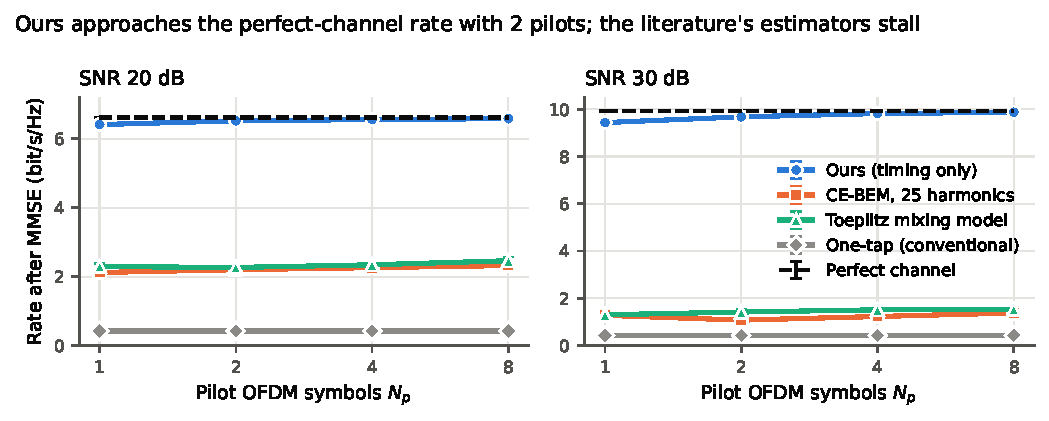
\includegraphics[width=\columnwidth]{fig1_estimators_vs_pilots.pdf}
\caption{Rate vs pilot symbols at 20 and 30\,dB, 20 channels with 95\% CIs.}
\label{fig:est}\end{figure}
\begin{figure}[t]\centering
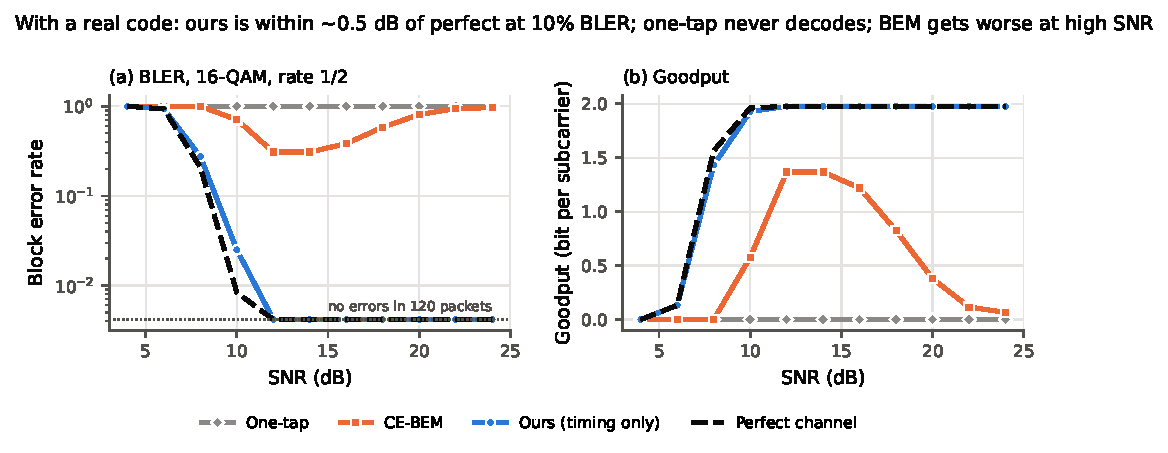
\includegraphics[width=\columnwidth]{fig15_coded_bler.pdf}
\caption{Coded block error rate and goodput, rate-1/2 convolutional code, 16-QAM.}
\label{fig:coded}\end{figure}
\begin{figure}[t]\centering
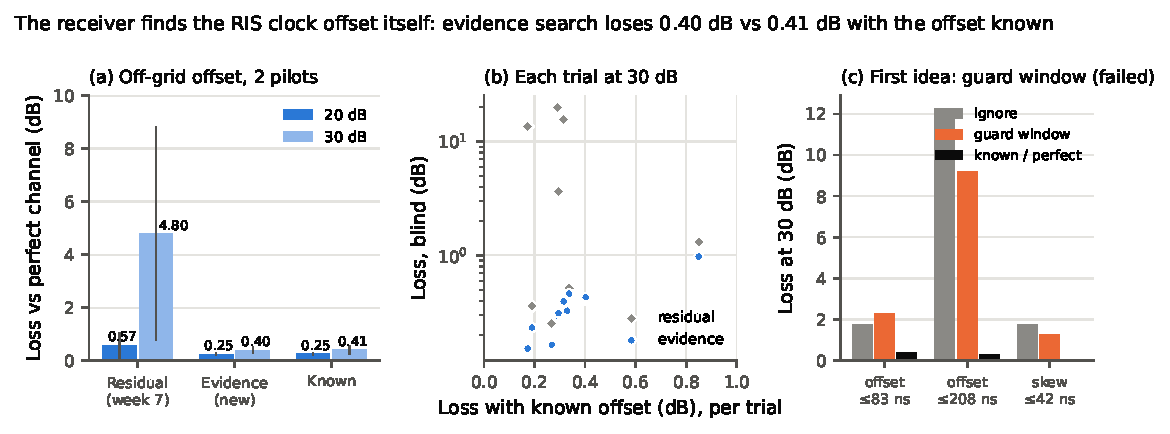
\includegraphics[width=\columnwidth]{fig20_blind_timing.pdf}
\caption{Blind recovery of an off-grid RIS clock offset from two pilot symbols.}
\label{fig:timing}\end{figure}
\begin{figure}[t]\centering
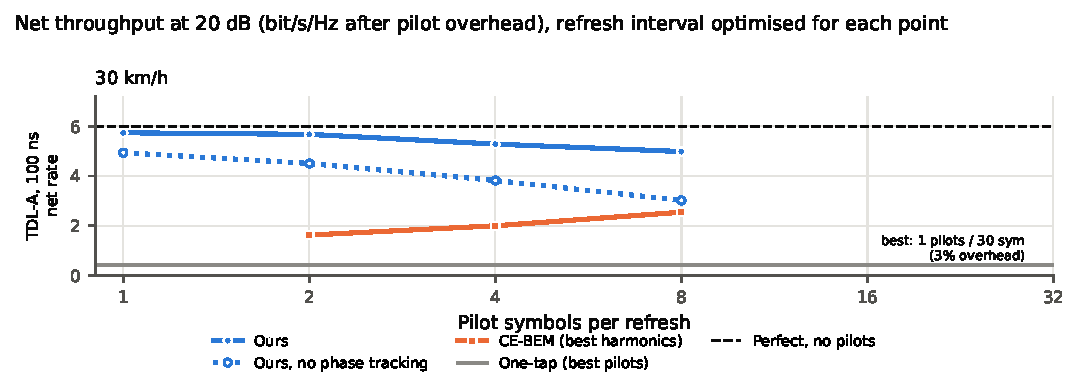
\includegraphics[width=\columnwidth]{fig19_pilot_overhead.pdf}
\caption{Net throughput after pilot overhead vs pilot symbols per refresh, 20\,dB.
\TODO{a two-row compact version for the letter (6-path and TDL-C).}}
\label{fig:overhead}\end{figure}

\emph{Limitations.} Results are simulated with one published element model and no
mutual coupling. At 120\,km/h a pilot is needed every $\sim$8 symbols; two tracking
receivers did not improve on this, and at 30\,dB the Doppler spread within a
symbol, not modelled here, limits every receiver. At 300\,ns delay spread the
static BS--RIS hop must be learned over $\sim$100 frames (TDL-A/C, gap
0.23--0.26\,bit/s/Hz at 20\,dB); channels whose taps exceed the cyclic prefix
are out of scope. % week8_twoscale_300ns_c.m, week8_tracking_120b.m

\section{Conclusion}
Grouping the TM-RIS harmonic expansion by state separates the control timing,
known at the receiver, from the element dispersion, which can be absorbed into the
unknown channel. A receiver built on this separation needs no element model,
finds the RIS clock offset by itself, equalizes without forming the coupling
matrix, and turns the harmonic coupling that conventional receivers suffer from
into usable rate.

\begin{thebibliography}{99}
\bibitem{iudice2026} I. Iudice, D. Darsena, G. Gelli, and V. Galdi, ``Physically consistent modeling of dispersive time-modulated reconfigurable intelligent surfaces for wideband OFDM,'' arXiv:2609.18360, Sep. 2026.
\bibitem{zhang2018} L. Zhang \emph{et al.}, ``Space-time-coding digital metasurfaces,'' \emph{Nat. Commun.}, vol. 9, art. 4334, 2018.
\bibitem{xu2023tmirs} \TODO{authors}, ``Time-modulated intelligent reflecting surface for waveform security,'' arXiv:2310.13210, 2023.
\bibitem{wang2026generative} K. Wang, S. Xiang, and A. Petropulu, ``Generative control of time-modulated intelligent reflecting surfaces for scalable directional modulation,'' arXiv:2610.12773, Oct. 2026.
\bibitem{hrycak2010} T. Hrycak, S. Das, G. Matz, and H. G. Feichtinger, ``Low complexity equalization for doubly selective channels modeled by a basis expansion,'' \emph{IEEE Trans. Signal Process.}, vol. 58, no. 11, pp. 5706--5719, Nov. 2010.
\bibitem{tang2007} Z. Tang, R. C. Cannizzaro, G. Leus, and P. Banelli, ``Pilot-assisted time-varying channel estimation for OFDM systems,'' \emph{IEEE Trans. Signal Process.}, vol. 55, no. 5, pp. 2226--2238, May 2007.
\bibitem{hu2019twotimescale} C. Hu and L. Dai \emph{et al.}, ``Two-timescale channel estimation for reconfigurable intelligent surface aided wireless communications,'' arXiv:1912.07990, 2019. \TODO{check full author list and journal version}
\bibitem{access2019bayes} \TODO{authors}, ``Bayesian model selection for OFDM channel estimation with residual timing offsets,'' \emph{IEEE Access}, 2019 (eprints.gla.ac.uk/188514). \TODO{check exact title}
\bibitem{chen2024sr} H. Chen, R. Long, Y.-C. Liang, and R. Schober, ``Blind timing estimation and signal detection for RIS-assisted symbiotic radio with imperfect symbol synchronization,'' in \emph{Proc. IEEE ICC}, 2024, pp. 4155--4160.
\bibitem{tr38901} 3GPP, ``Study on channel model for frequencies from 0.5 to 100 GHz,'' TR 38.901.
\end{thebibliography}
\end{document}
